%This file was the "original" raster calibration document I wrote. It has been updated since. Keeping this file around for a while in case I need something from it. The new document will be an appendix.

\iffalse In order to accurately determine the position of the beam, the raster needs to be calibrated to the BPMs. Reading out the BPMs gives an accurate position, but it has a phase lag which causes the readout to be uncorrelated with the events it is recorded with. The raster current is read instantaneously, which means it is an accurate for the event it is recorded with. However, the raster current does not directly tell us the position of the beam. Using these two systems together, the BPMs give the spread of the beam and the raster current can then be mapped to this spread. When the transformation between the raster current and position is found, it is easy to have an accurate beam position for every event that is recorded.

\begin{figure}
	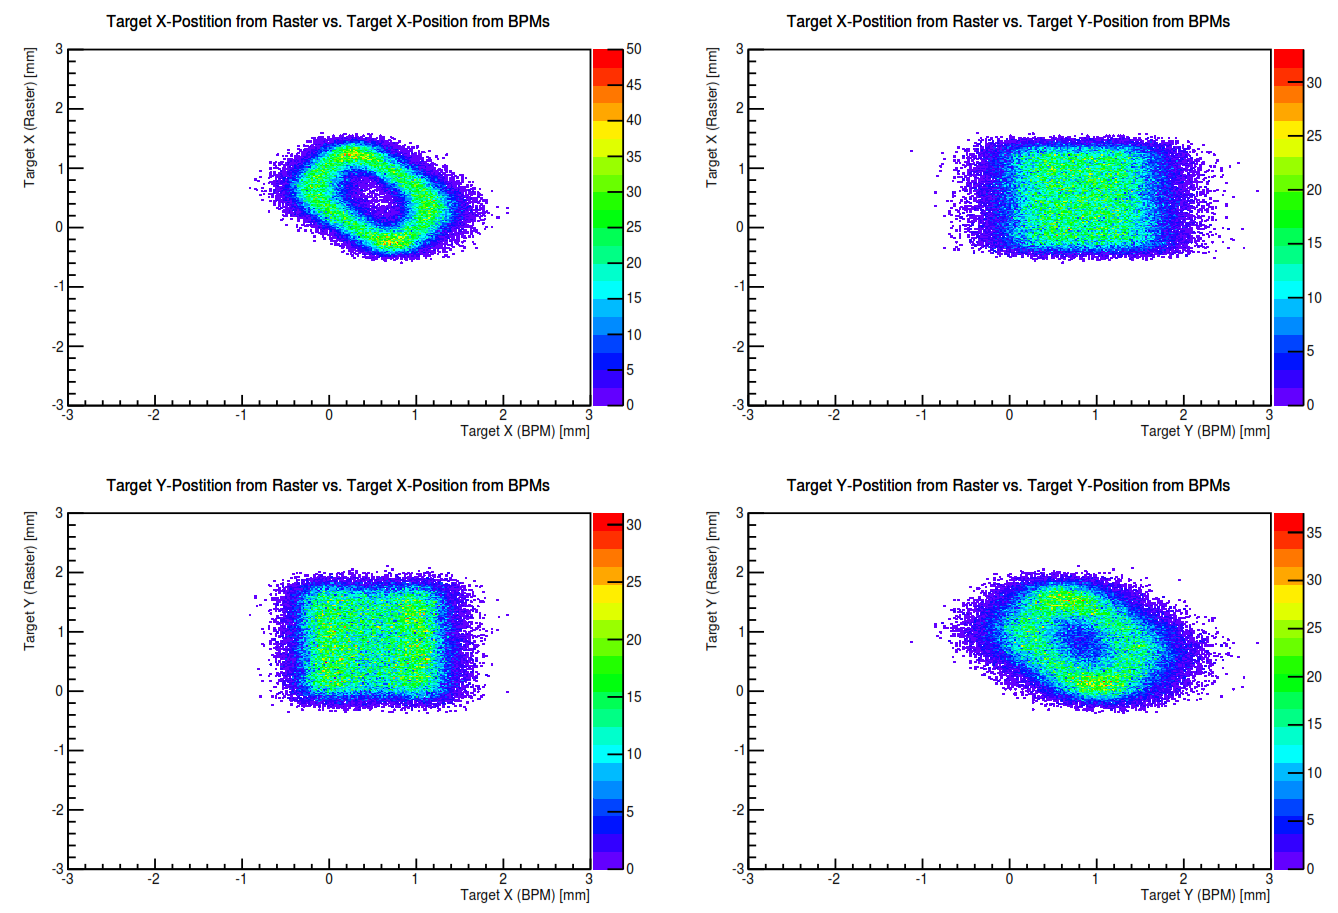
\includegraphics[width=\linewidth]{./analysis/fig/raster_bpm_sync.png}
	\caption{The BPM has a phase lag, causing the raster and BPMs to not be synced}
	\label{fig:rastersync}
\end{figure}
\fi

A well calibrated raster will map a raster current to the instantaneous beam position on the target. Accurate beam position data is critical for proper reconstruction of the reaction vertex of physics events. A poorly calibrated horizontal raster will cause poor z-vertex resolution, making it more difficult to subtract the background from target endcaps. A poorly calibrated vertical raster will incorrectly reconstruct event momentum, causing errors in physics analysis.

In Hall A, we have two sets of raster coils working in tandem for the 12 GeV era. Each set of raster coils are synced to ensure that they work together, always steering the beam in the same direction. With this knowledge, the Hall A Analyzer is set up so that the signals from a single raster set are used to determine the beam position. In our case, the analysis code is set up to use the upstream raster coils.

The raster calibration can be thought of as defining a line that maps the raster current (measured in ADC bins) to a position on the target. Each coil will have two calibration values, the slope and intercept of this line. The slope of the line determines the size calibration of the raster coil, the value converts the raster current (in ADC units) to a beam position displaced about the mean beam position. The intercept of the line, in conjunction with the slope, sets this mean beam position.

In the past, these values have been found by assuming that the BPMs accurately reflect the mean position and overall magnitude of the rastered beam. By mapping the mean and extremes of raster current to the mean and extremes of BPM positions, a 1:1 mapping could be quickly achieved. Unfortunately, in the Tritium era of Hall A, we have seen that the BPMs no longer accurately reflect the magnitude of the rastered beam. An explanation of this behavior has not been found. Nevertheless, we must find a new calibration method.

While the BPMs can (and still are) used to determine the mean beam position, we must look for other quantities to calibrate the raster size. The obvious choice is the carbon hole target. The carbon hole is used to set the size during data taking because it is known to have a diameter of 2mm. The hole is visible in the raster spectrum, so we can fit it to determine a size calibration for the raster.

The resolution of reconstructed events does not allow for a hard line between the events originating from the foil and the absence of events in the "hole" region. Events smear across this border suggesting that we ought to use a smooth function to define the edge. I decided to use a radial sigmoid function with a floating "hardness" constant. A sigmoid is a smoothed step function with a constant that determines how hard of a step it is. As shown in Figure \ref{fig:sighard}, a sigmoid approaches a step function as the "hardness" constant approaches infinity. This was found to converge\footnote{When doing these fits, be sure to the Log Likelihood method} and visually appears to fit the hole well. This fitting procedure determines the edge of the hole to be at the position where the value is halfway between the minimum and maximum value of function.

\begin{figure}
	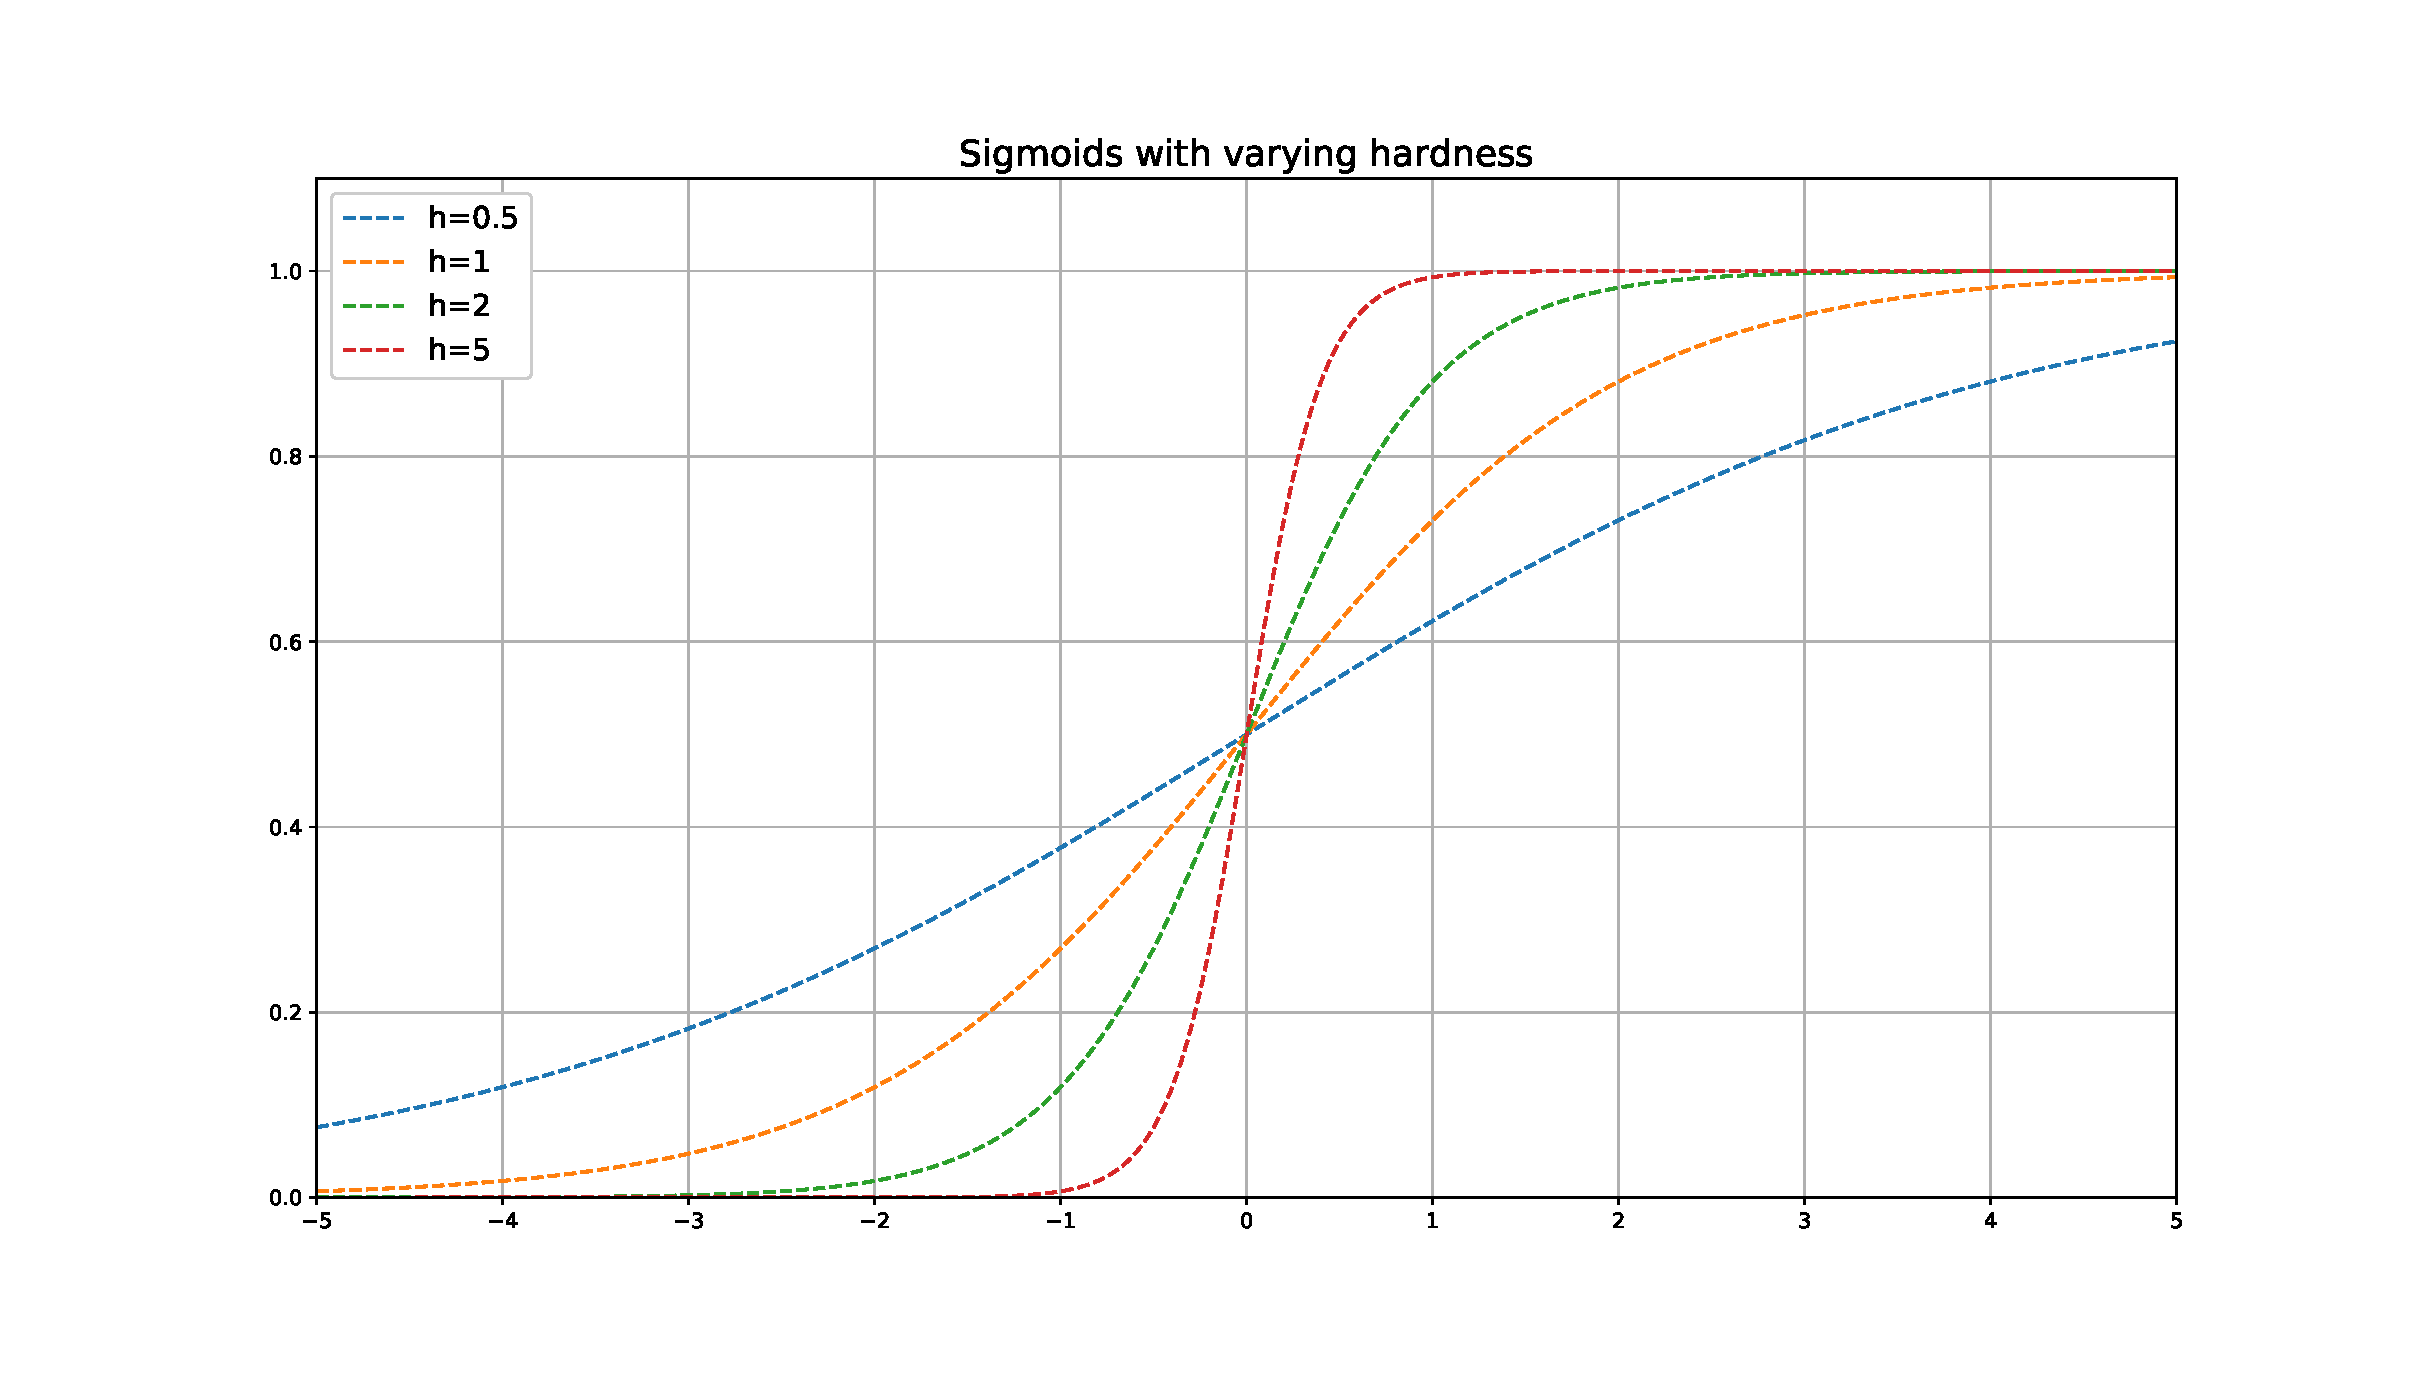
\includegraphics[width=\textwidth]{./analysis/fig/sig_hard.eps}
	\caption{A 1 Dimensional Sigmoid Function with Varying Hardness Parameter}
	\label{fig:sighard}
\end{figure}

The function used is:
\begin{equation}
\frac{[0]}{1+e^{-[5]*\left(\left([1]*\left([2]-x\right)\right)^{2}+\left([3]*\left([4]-y\right)\right)^{2}-1\right)}}+[6]
\label{eqn:radsig}
\end{equation}

In this function:

\begin{center}
\begin{tabulary}{\textwidth}{|L|L|}
	\multicolumn{2}{c}{\textbf{Variable Definitions}}
	\\
	\hline
	$[0]$ & Approximate signal level outside the carbon hole (measured in ADC bins)\\
	$[1]$ & Current (ADC) to size conversion factor for Horizontal Raster\\
	$[2]$ & Horizontal center of the carbon hole in current (ADC) units\\
	$[3]$ & Current (ADC) to size conversion factor for Vertical Raster\\
	$[4]$ & Vertical center of the carbon hole in current (ADC) units\\
	$[5]$ & "Hardness" factor for the sigmoid (approaches a step function as this increases)\\
	$[6]$ & Approximate signal level inside the carbon hole (measured in ADC bins)\\
	\hline
\end{tabulary}
\end{center}

\begin{figure}
	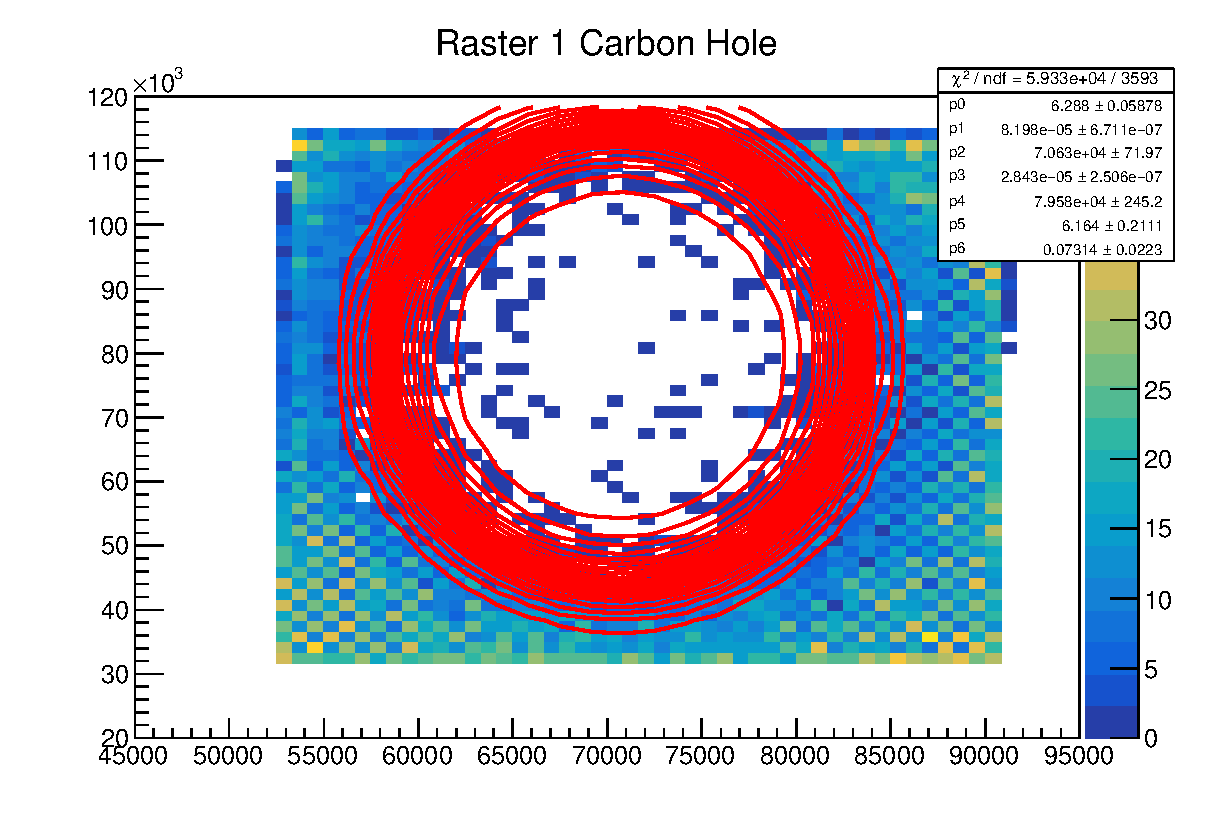
\includegraphics[width=\textwidth]{./analysis/fig/final_chole_fit.eps}
	\caption{Using the radial sigmoid function to fit the hole in the Carbon Hole target. In this plot, the density of red rings is directly correlated to the slope of the function at that point. Where the rings are densest is the 50\% position, corresponding to where the fit locates the edge of the hole.}
	\label{fig:carbholefit}
\end{figure}

Upon further analysis it was determined that the calibration was not good. The fit places the edge of the hole at the zero-crossing of the sigmoid function. Due to smearing from the spectrometer, this is not the "true edge" of the hole.

Proceeding further, we determined that we ought to look at the physics values that the raster calibration affects. For the horizontal rasters, this is the reconstructed z position at the target. For the vertical rasters, this is W$^2$. By utilizing two "bad" calibrations, we can interpolate (or extrapolate if they were bad in the same direction) to determine the correct calibration.

For the horizontal raster, we use the single carbon foil target and plot the horizontal raster current versus the reconstructed z position. We can then take slices of this plot in horizontal raster current bins and fit the resulting plots with a Gaussian and plot the peaks. With a properly calibrated raster, there should be no correlation between horizontal raster current and reconstructed z. Using two improper horizontal calibrations, we measured the slopes of the correlations. We then interpolated to determine the calibration that would yield a slope of 0.

In practice, this does not yield a calibration with a slope of \textit{precisely} zero. This is due to statistical fluctuations in the data around the true correlation line. We attempted to iterate this procedure, but it did not yield significant improvement on the results.

\begin{figure}
	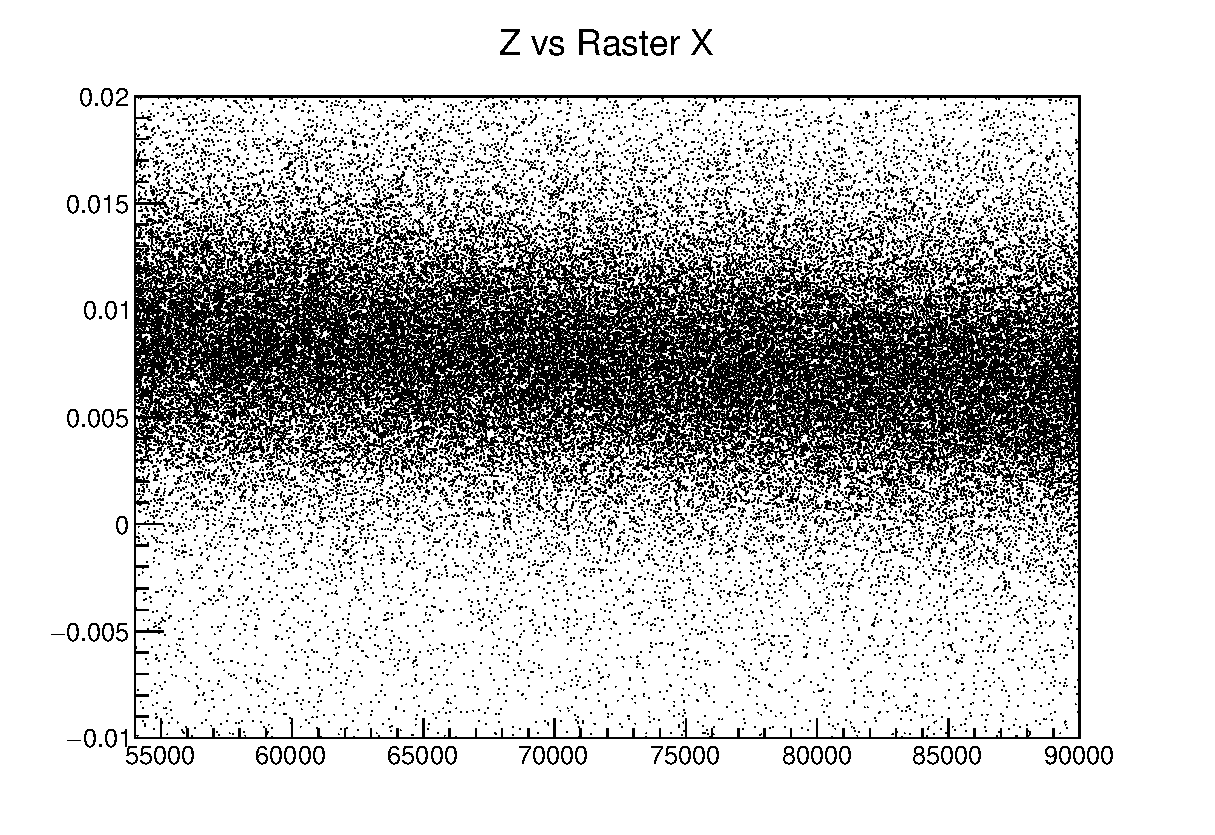
\includegraphics[width=\textwidth]{./analysis/fig/old1_zvx.eps}
	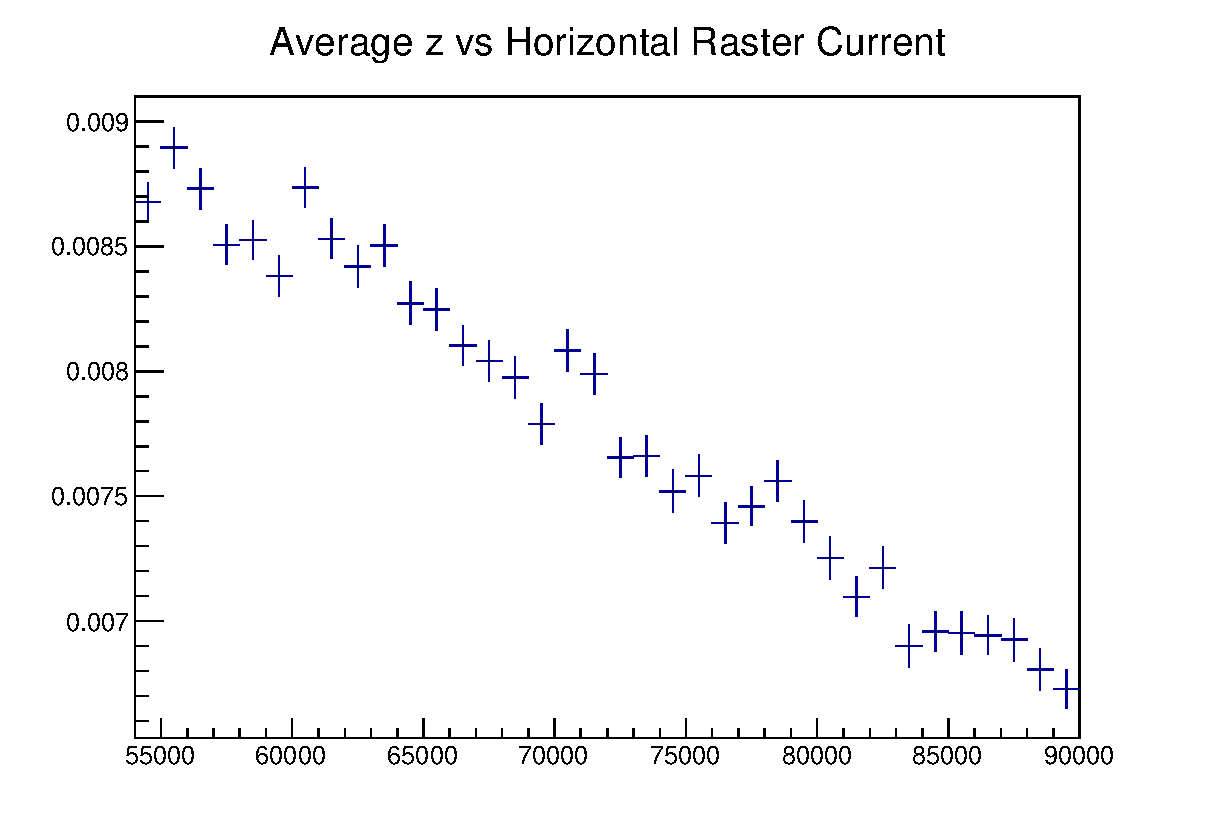
\includegraphics[width=\textwidth]{./analysis/fig/old1_avgz_nofit.eps}
	\caption{Slices in horizontal raster current of the reconstructed z versus raster current plot are fit with a Gaussian. The peaks of the Gaussian are then plot to see the correlation. In the plot of average z, it can be seen that the peak position shifts by over 2mm over the movement of the raster. The carbon foil is only 0.25mm thick.}
\end{figure}

\begin{figure}
	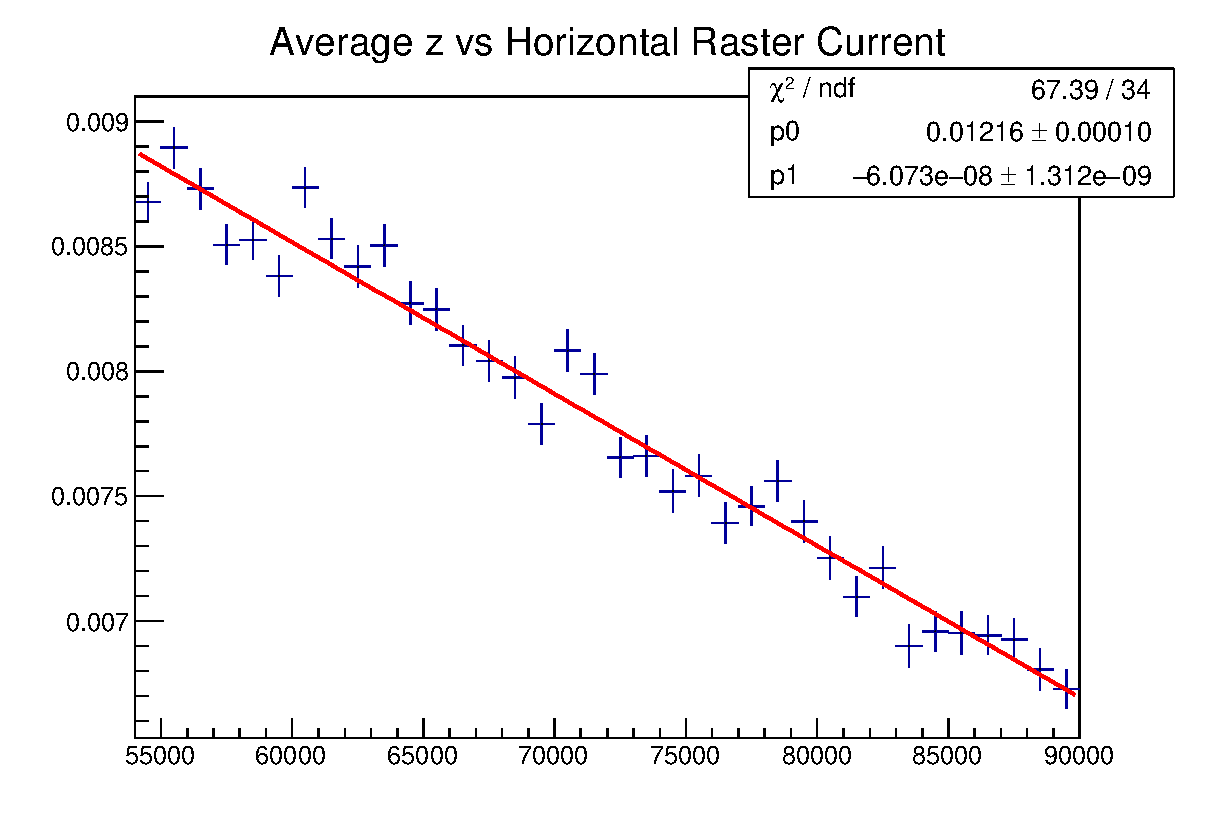
\includegraphics[width=\textwidth]{./analysis/fig/old1_avgz.eps}
	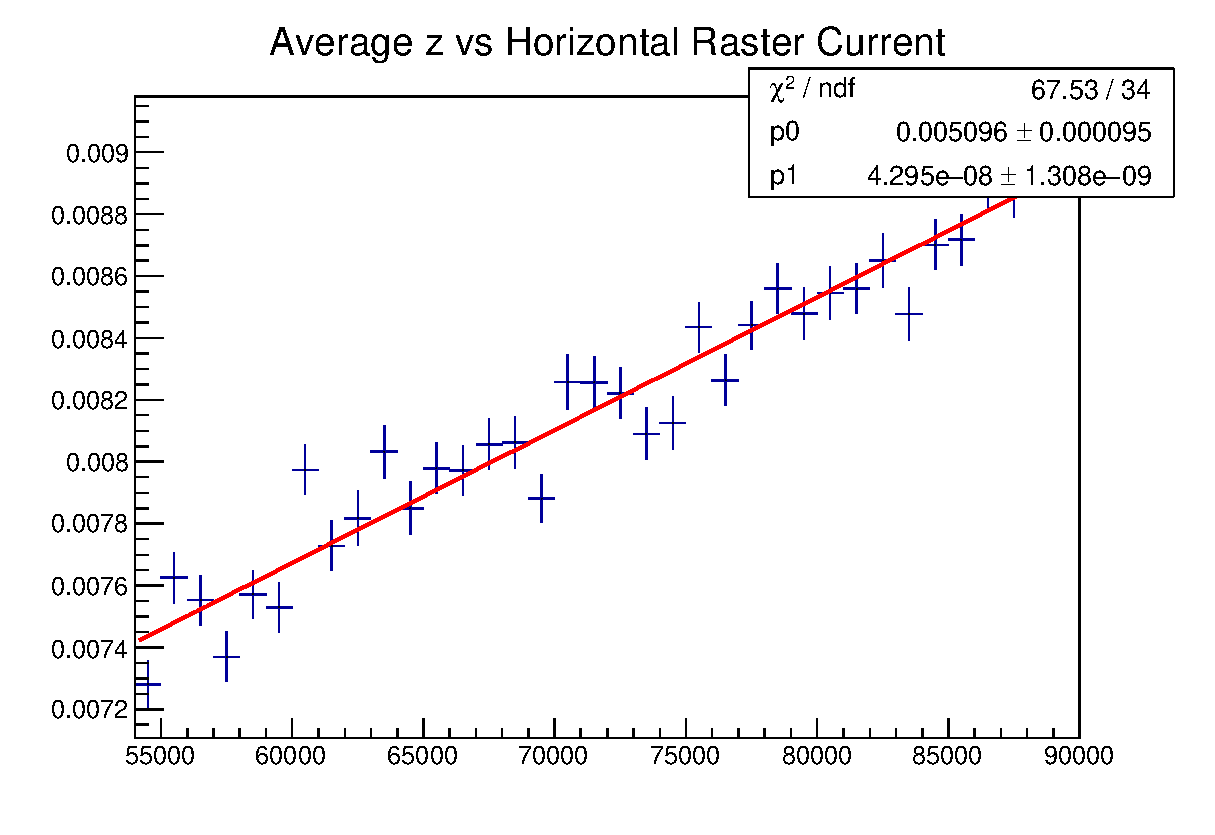
\includegraphics[width=\textwidth]{./analysis/fig/old2_avgz.eps}
	\caption{Two "bad" calibrations are fit to find the correlation between horizontal raster current and the average x position. Both of these calibrations show a displacement larger than the thickness of the target.}
\end{figure}
\begin{figure}
	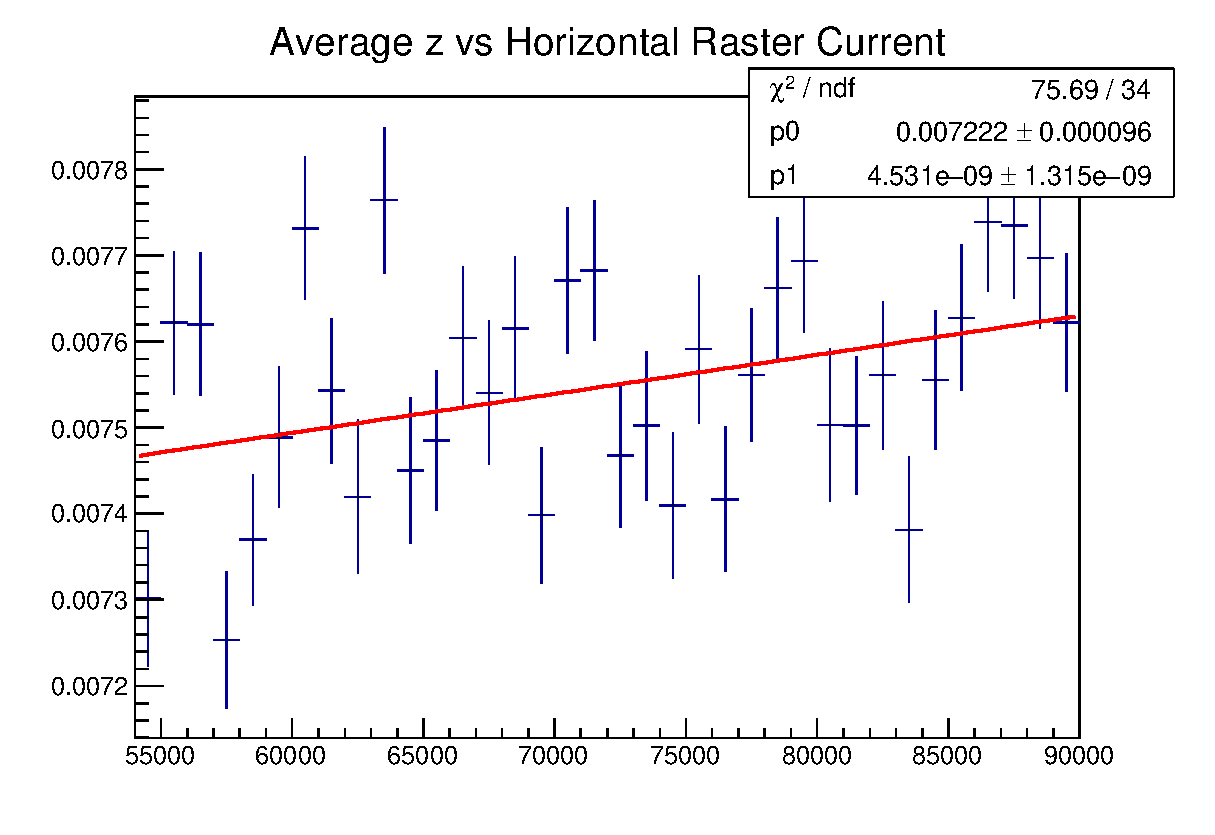
\includegraphics[width=\textwidth]{./analysis/fig/final_avgz.eps}
	\caption{Using a linear fit of the correlation between average z and horizontal raster current for two "bad" calibrations, we can interpolate to the correct calibration. Here we can see that the shift is approximately 0.1mm.}
\end{figure}

For the vertical raster, we look for a momentum feature that the experiment can see. In the case of many of the Tritium era experiments, the Hydrogen elastic peak was measured. Plotting the vertical raster current versus the W$^2$ of Hydrogen elastic events, we followed a similar procedure to that of the horizontal raster.

For experiments that do not have an identifiable momentum feature, an approximation of the correct vertical calibration can be found using the horizontal calibration and the sigmoid fit of the carbon hole. Since it is known that the true calibration lies somewhere on the sigmoid above the zero-crossing, we can use the horizontal calibration to determine where that point is. To do this, we determine how many horizontal ADC bins away from center the "true edge" lies using the calibration determined using the z vertex reconstruction (the "true edge" is $1mm$ away from the center). We then evaluate equation \ref{eqn:radsig} using this value. Then, equation \ref{eqn:radsig} is reversed to determine the vertical ADC bin displacement to yield the same value. Once we have the displacement, a new vertical calibration can be determined. This is an imperfect solution, but ultimately should provide the best calibration possible in the absence of a momentum feature.

Once these methods are used to determine the slope of the raster calibration, we turn our attention back to the BPMs. The BPMs, after calibration with the harp, provide a very accurate reading of the mean beam position at their location in the beamline. This information can then be used to determine the mean position of the beam at the target. To do this, we plot each BPMs position spectrums and determine the mean value. Each spectrum must have its mean determined independently because the BPM readings lag behind events, the position is only accurate when averaged over time. Once we know the mean positions at each BPM, a track through the means can be projected to the mean position at the target.

With the slope of the raster calibrations and a point on the calibration lines (the mean position at the target), we have all the information that we need to determine the raster calibration lines. Using a simple point-slope form, we input the information for each raster and solve for the intercept.